%%%%%%%%%%%%%%%%%%%%%%%%%%%%%%%%%%%%%%%%%%%%%%%%%%%%%%%%%%%%%%%%%%%%%%%%%%%%%%%
%                       CARREGA DE LA CLASSE DE DOCUMENT                      %
%                                                                             %
% Les opcions admissibles son:                                                %
%      12pt / 11pt            (cos dels tipus de lletra; no feu servir 10pt)  %
%                                                                             %
% catalan/spanish/english     (llengua principal del treball)                 %
%                                                                             % 
% french/italian/german...    (si necessiteu fer servir alguna altra llengua) %
%                                                                             %
% listoffigures               (El document inclou un Index de figures)        %
% listoftables                (El document inclou un Index de taules)         %
% listofquadres               (El document inclou un Index de quadres)        %
% listofalgorithms            (El document inclou un Index d'algorismes)      %
%                                                                             %
%%%%%%%%%%%%%%%%%%%%%%%%%%%%%%%%%%%%%%%%%%%%%%%%%%%%%%%%%%%%%%%%%%%%%%%%%%%%%%%

\documentclass[11pt,spanish,listoffigures,listoftables]{workluis}

%%%%%%%%%%%%%%%%%%%%%%%%%%%%%%%%%%%%%%%%%%%%%%%%%%%%%%%%%%%%%%%%%%%%%%%%%%%%%%%
%                     CODIFICACIO DEL FITXER FONT                             %
%                                                                             %
%    windows fa servir normalment 'ansinew'                                   %
%    amb linux es possible que siga 'latin1' o 'latin9'                       %
%    Pero el mes recomanable es fer servir utf8 (unicode 8)                   %
%                                          (si el vostre editor ho permet)    % 
%%%%%%%%%%%%%%%%%%%%%%%%%%%%%%%%%%%%%%%%%%%%%%%%%%%%%%%%%%%%%%%%%%%%%%%%%%%%%%%

\usepackage[utf8]{inputenc} 

%%%%%%%%%%%%%%%%%%%%%%%%%%%%%%%%%%%%%%%%%%%%%%%%%%%%%%%%%%%%%%%%%%%%%%%%%%%%%%%
%                        ALTRES PAQUETS I DEFINICIONS                         %
%                                                                             %
% Carregueu aci els paquets que necessiteu i declareu les comandes i entorns  %
%                                          (aquesta seccio pot ser buida)     %
%%%%%%%%%%%%%%%%%%%%%%%%%%%%%%%%%%%%%%%%%%%%%%%%%%%%%%%%%%%%%%%%%%%%%%%%%%%%%%%



%%%%%%%%%%%%%%%%%%%%%%%%%%%%%%%%%%%%%%%%%%%%%%%%%%%%%%%%%%%%%%%%%%%%%%%%%%%%%%%
%                        DADES DEL TREBALL                                    %
%                                                                             %
% titol, alumne, tutor i curs academic                                        %
%%%%%%%%%%%%%%%%%%%%%%%%%%%%%%%%%%%%%%%%%%%%%%%%%%%%%%%%%%%%%%%%%%%%%%%%%%%%%%%

\title{Problema de clasificación \\
         Vehicle silhouettes}
\author{Luis Cabrero García}
\tutor{José María Valls Ferrán}
\curs{4º - Gr80}

%%%%%%%%%%%%%%%%%%%%%%%%%%%%%%%%%%%%%%%%%%%%%%%%%%%%%%%%%%%%%%%%%%%%%%%%%%%%%%%
%                              INICI DEL DOCUMENT                             %
%%%%%%%%%%%%%%%%%%%%%%%%%%%%%%%%%%%%%%%%%%%%%%%%%%%%%%%%%%%%%%%%%%%%%%%%%%%%%%%

\begin{document}

%%%%%%%%%%%%%%%%%%%%%%%%%%%%%%%%%%%%%%%%%%%%%%%%%%%%%%%%%%%%%%%%%%%%%%%%%%%%%%%
%              RESUMS DEL TFG EN VALENCIA, CASTELLA I ANGLES                  %
%%%%%%%%%%%%%%%%%%%%%%%%%%%%%%%%%%%%%%%%%%%%%%%%%%%%%%%%%%%%%%%%%%%%%%%%%%%%%%%

\makeindexes

%%%%%%%%%%%%%%%%%%%%%%%%%%%%%%%%%%%%%%%%%%%%%%%%%%%%%%%%%%%%%%%%%%%%%%%%%%%%%%%
%                              CONTINGUT DEL TREBALL                          %
%%%%%%%%%%%%%%%%%%%%%%%%%%%%%%%%%%%%%%%%%%%%%%%%%%%%%%%%%%%%%%%%%%%%%%%%%%%%%%%

\mainmatter

%%%%%%%%%%%%%%%%%%%%%%%%%%%%%%%%%%%%%%%%%%%%%%%%%%%%%%%%%%%%%%%%%%%%%%%%%%%%%%%
%                                  INTRODUCCIÓN                               %
%%%%%%%%%%%%%%%%%%%%%%%%%%%%%%%%%%%%%%%%%%%%%%%%%%%%%%%%%%%%%%%%%%%%%%%%%%%%%%%

\chapter{Introducci\'on}

\par La presente práctica trata de abordar mediante el punto de vista de las redes de neuronas supervisadas y no supervisadas la resolución de un problema real: la clasificación de determinadas siluetas de vehículos en cuatro tipos dados. Estos datos han sido tomados del KEEL\cite{KEEL}.

\section{Motivaci\'on}

\par La utilidad de los modelos de clasificación que vamos a aplicar de forma práctica es reseñable: nos permiten determinar la categoría a la que pertenece un vehículo determinado a partir de sus características, resultando de gran interés y aplicable a problemas reales.

\section{Objetivos}

\par Los objetivos de la práctica son: procesar y preparar los datos del KEEL\cite{KEEL} para validación cruzada estratificada, clasificar los datos utilizando el Perceptrón Multicapa, clasificar los datos utilizando LVQ, y por último, utilizando mapas autoorganizados de Kohonen. Posteriormente se hará una comparación entre los tres modelos para ver en que casos unos modelos pueden clasificar mejor que otros.

\section{Estructura de la memoria}

\par La memoria dispone de tres índices, uno para consultar cada una de las secciones y otros dos para figuras y tablas. En la memoria se puede encontrar tres apartados generales para el modelo MLP, LVQ y mapas de Kohonen. Dentro de los respectivos apartados de cada modelo, se explica la base teórica de cada uno de ellos, se explican los distintos experimentos realizados y se comparan los resultados en función de los parámetros escogidos. En las conclusiones se explican las diferencias entre los modelos y se comparan los resultados obtenidos en la experimentación. Al final de la memoria se indican las referencias bibliográficas consultadas para llevar a cabo el trabajo.

%\section{Notes bibliografiques} %%%%% Opcional

%????? ????????????? ????????????? ????????????? ????????????? ?????????????

%%%%%%%%%%%%%%%%%%%%%%%%%%%%%%%%%%%%%%%%%%%%%%%%%%%%%%%%%%%%%%%%%%%%%%%%%%%%%%%
%                         CAPITOLS (tants com calga)                          %
%%%%%%%%%%%%%%%%%%%%%%%%%%%%%%%%%%%%%%%%%%%%%%%%%%%%%%%%%%%%%%%%%%%%%%%%%%%%%%%

%%%%%%%%%%%%%%%%%%%%%%%%%%%%%%%%%%%%%%%%%%%%%%%%%%%%%%%%%%%%%%%%%%%%%%%%%%%%%%%
%                           PREPARACIÓN DE LOS DATOS                          %
%%%%%%%%%%%%%%%%%%%%%%%%%%%%%%%%%%%%%%%%%%%%%%%%%%%%%%%%%%%%%%%%%%%%%%%%%%%%%%%

\chapter{Preparación de los datos}

\section{Clasificación de los datos}

\par En este capítulo se va a explicar la preparación de los datos que se ha llevado a cabo para poder posteriormente aplicar los diferentes modelos.

\par Lo primero que se hace con los datos es separarlos en cuatro hojas, cada una de ellas correspondiente con cada una de las clases existentes: bus, van, saab y opel. Posteriormente lo que se hace es formar tres conjuntos de datos: P1, P2 y P3, que serán otras tres hojas de datos. En cada uno de los tres conjuntos de datos se introducen una tercera parte de los datos de cada una de las clases.

\section{Preparación de los conjuntos de entrenamiento y test}

\par Una vez tenemos los datos originales repartidos en los tres conjuntos de datos, lo que debemos hacer es distribuir estos conjuntos para formar 3 parejas de conjuntos de entrenamiento y test. El proceso para formar estos ficheros es ir copiando los datos de los conjuntos P1, P2 y P3, en distintas combinaciones para poder formar los conjuntos.

\section{Normalización de los conjuntos de entrenamiento y test}

\par Cuando se dispone de los conjuntos de entrenamiento y test lo que se debe hacer es normalizar los datos en función de los valores máximo y mínimo del conjunto original. Para ello se aplica la siguiente fórmula:
\begin{equation}\label{eq:ej}
Valor_{normalizado} = \frac{V_{original} - Valor_{min}}{Valor_{max} - Valor_{min}}
\end{equation}

\par Una vez hemos normalizado todos los datos de \textbf{todos} los conjuntos de entrenamiento y test, debemos desordenar los patrones de entrenamiento para presentárselos a nuestros modelos. Esto lo conseguimos añadiendo una columna aleatoria y ordenando posteriormente por esa columna.

%%%%%%%%%%%%%%%%%%%%%%%%%%%%%%%%%%%%%%%%%%%%%%%%%%%%%%%%%%%%%%%%%%%%%%%%%%%%%%%
%                           PERCEPTRÓN MULTICAPA MLP                          %
%%%%%%%%%%%%%%%%%%%%%%%%%%%%%%%%%%%%%%%%%%%%%%%%%%%%%%%%%%%%%%%%%%%%%%%%%%%%%%%

\chapter{Perceptrón Multicapa}

\par En este capítulo se va a explicar en primer lugar el modelo Perceptrón Multicapa, que sirve para solucionar problemas de clasificación, es decir, estableciendo una correspondencia entre un conjunto de datos y un conjunto de clases determinadas. Para poder afrontar el problema necesitamos conocer el número de clases. Si el número de clases es desconocido entonces es necesario utilizar redes de neuronas no supervisadas, que serán abordadas en los próximos capítulos.

\section{Perceptron Multicapa (MLP)}

\par Es una red de neuronas artificiales formada por múltiples capas (\ref{fig:mlp}) que resuelve problemas que no son linealmente separables. Además, se ha demostrado que es un aproximador universal, es decir,  cualquier función contínua en el espacio $\mathbb{R}^n$ puede aproximarse con este modelo. 

\begin{figure}[H]
\centering
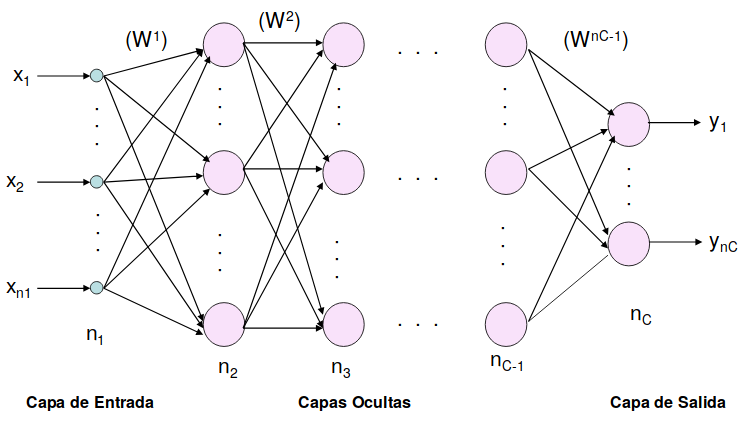
\includegraphics[scale=0.5]{mlp}
\caption{Red Perceptrón multicapa \cite{MLP}}\label{fig:mlp}
\end{figure}

\par La arquitectura está distribuida en tres tipos de neuronas: neuronas de entrada, que únicamente reciben las entradas y las propagan a la siguiente capa, las neuronas ocultas, que procesan de manera no lineal las entradas, y las neuronas de salida, que devuelven las salidas al exterior.

\par Teniendo dos neuronas \textit{i} y \textit{j}:

\begin{figure}[H]
\centering
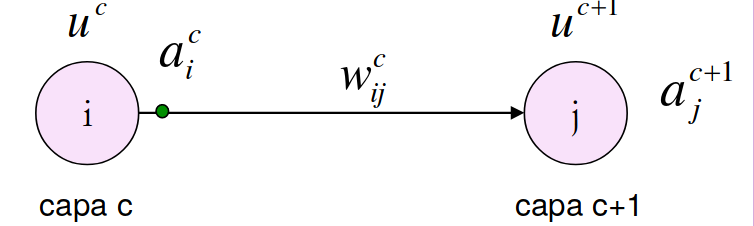
\includegraphics[scale=0.3]{mlpesquema}
\caption{Esquema MLP \cite{MLP}}\label{fig:esquema}
\end{figure}

\par Los pesos y el umbral (\ref{eq:ej6}) se expresan en forma matricial, e influyen en la activación de la neurona perteneciente a la capa siguiente. Las neuronas de entrada simplemente tienen su activación equivalente a la entrada que reciben, sin embargo, tanto las neuronas de la capa de salida (\ref{eq:ej8}) como las neuronas de las capas ocultas (\ref{eq:ej7}) necesitan computar los pesos y sus entradas sumándoles el umbral.

\begin{equation}\label{eq:ej6}
W^c = (w_{ij}^c) = \begin{pmatrix}
w_{11}^c & w_{12}^c & ... & w_{1n_{c+1}}^c\\ 
w_{21}^c & w_{22}^c & ... & w_{2n_{c+1}}^c\\ 
... & ... & & ...\\ 
w_{n_{c}1}^c & w_{n_{c}2}^c & ... & w_{n_{c}n_{c+1}}^c 
\end{pmatrix}  ,  U^c = (u_{i}^c) = \begin{pmatrix}
u_{1}^c\\ 
u_{2}^c\\ 
...\\ 
u_{n_{c}}^c 
\end{pmatrix}
\end{equation}

\begin{equation}\label{eq:ej7}
a_{i}^c = f(\sum_{j=1}^{n_{c-1}}w_{ji}^{c-1}*a_{j}^{c-1} + u_{i}^{c})
\end{equation} 

\begin{equation}\label{eq:ej8}
y_{i} = a_{i}^c = f(\sum_{j=1}^{n_{c-1}}w_{ji}^{c-1}*a_{j}^{c-1} + u_{i}^{c})
\end{equation} 

\par Siendo $f$ la función de activación. Las funciones más utilizadas son la función sigmoidal ($f_{1}(x) = \frac{1}{1+e^{-x}}$) y la tangente hiperbólica ($f_{2}(x) = \frac{1-e^{-x}}{1+e^{-x}}$). El aprendizaje de la red se realiza de forma semejante que en Adaline \cite{MLP}.

\section{Script en RSNNS}

\par Para realizar la experimentación se proporciona un script que realiza los siguientes pasos:

\begin{itemize}
\item Se cargan dos ficheros de entrenamiento y test que forman una pareja. Posteriormente se cargan los ficheros correspondientes a las otras dos parejas, teniendo de esta manera la validación cruzada.
\item Se codifican las cuatro clases (bus, van, saab y opel) en 4 números.
\item Se seleccionan los parámetros: razón de aprendizaje, topología de la red y ciclos.
\item Se ejecuta el aprendizaje y se selecciona el modelo.
\item Se muestra en un gráfico la evolución del error (SSE) según avanzan los ciclos.
\item Se generan matrices de confusión que muestran los valores predichos frente a los reales.
\item Se halla el porcentaje de acierto.
\item Se expresa en una tabla los errores por ciclo.
\item Se calcula el error final MSE.
\item Se guardan los resultados en ficheros.
\end{itemize}

\section{Experimentación realizada}

\par En cuanto a la experimentación realizada se ha prestado especial atención en conseguir una capacidad de generalización adecuada. Esto es: no nos interesa conseguir que la red sea capaz de estimar valores del conjunto de entrenamiento pero que cuando entren datos de un conjunto nuevo, no sea capaz de generalizarlos. Esta situación es conocida como \textbf{sobreaprendizaje}. Para cada uno de los experimentos realizados, será de especial interés observar la matriz de confusión para ver las predicciones que hace el modelo frente a los valores reales.

\par \underline{\textbf{Experimentaciones}}

%   EXPERIMENTO 1    %

\par \textbf{$\gamma = 0.1$, $neuronas = 100$ y $ciclos = 10000$}

\par Con una tasa de 0.1, 100 neuronas en una capa oculta y 10000 ciclos tenemos los siguientes porcentajes de acierto:

\begin{table}[H]
\centering
\caption{MLP $\gamma = 0.1$, $neuronas = 100$ y $ciclos = 10000$}
\label{tb:tb1}
\begin{tabular}{lllll}
\hline
\multicolumn{1}{|l|}{Pareja} & Porcentaje de acierto entrenamiento & Porcentaje de acierto test  \\ \hline \hline
1                            & 0.913357400722022    & 0.215753424657534 \\
2                            & 0.760907504363002    & 0.754578754578755 \\
3                            & 0.783595113438045    & 0.825622775800712 \\
Media                        & 0.81928667333        & 0.59865165167     \\ \hline
\end{tabular}
\end{table}

\begin{figure}[H]
\centering
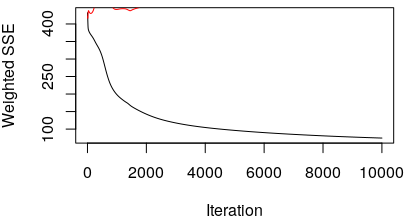
\includegraphics[scale=5]{011001}
\caption{MLP $\gamma = 0.1$, $neuronas = 100$ y $ciclos = 10000$ pareja 1}
\end{figure} 

\begin{figure}[H]
\centering
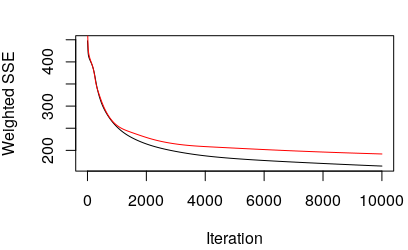
\includegraphics[scale=5]{011002}
\caption{MLP $\gamma = 0.1$, $neuronas = 100$ y $ciclos = 10000$ pareja 2}
\end{figure} 

\begin{figure}[H]
\centering
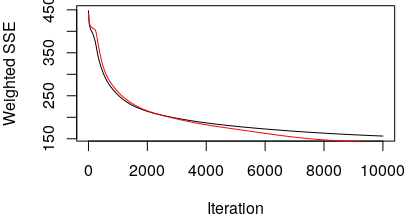
\includegraphics[scale=5]{011003}
\caption{MLP $\gamma = 0.1$, $neuronas = 100$ y $ciclos = 10000$ pareja 3}
\end{figure} 

\par Como se puede apreciar en las figuras, los resultados son bastante diferentes, la pareja 2 y 3 se aproxima bastante bien pero la primera pareja presenta resultados muy diferentes. La media del porcentaje de acierto es bastante bueno para entrenamiento pero no muy buena para test. Observando las matrices de confusión, la predicción no es muy buena para varias clases.

%   EXPERIMENTO 2    %

\par \textbf{$\gamma = 0.1$, $neuronas = 100,50$ y $ciclos = 1000$}

\par Con una tasa de 0.1, 100 neuronas y 50 neuronas distribuidas en dos capas ocultas y 10000 ciclos tenemos los siguientes porcentajes de acierto:

\begin{table}[H]
\centering
\caption{MLP $\gamma = 0.1$, $neuronas = 100,50$ y $ciclos = 1000$}
\label{tb:tb2}
\begin{tabular}{lllll}
\hline
\multicolumn{1}{|l|}{Pareja} & Porcentaje de acierto entrenamiento & Porcentaje de acierto test  \\ \hline \hline
1                            & 0.667870036101083    & 0.469178082191781 \\
2                            & 0.614310645724258    & 0.600732600732601 \\
3                            & 0.633507853403141    & 0.619217081850534 \\
Media                        & 0.63856284666        & 0.56304258825     \\ \hline
\end{tabular}
\end{table}

\begin{figure}[H]
\centering
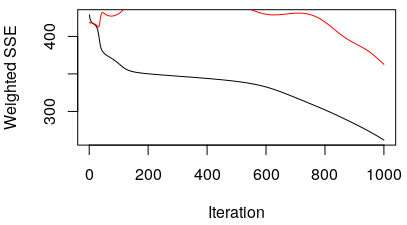
\includegraphics[scale=0.5]{01100501}
\caption{MLP $\gamma = 0.1$, $neuronas = 100,50$ y $ciclos = 1000$ pareja 1}
\end{figure} 

\begin{figure}[H]
\centering
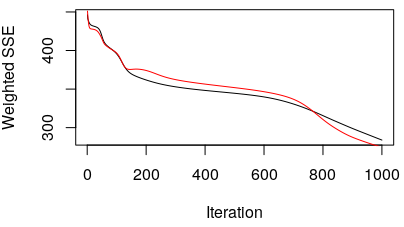
\includegraphics[scale=0.5]{01100502}
\caption{MLP $\gamma = 0.1$, $neuronas = 100,50$ y $ciclos = 1000$ pareja 2}
\end{figure} 

\begin{figure}[H]
\centering
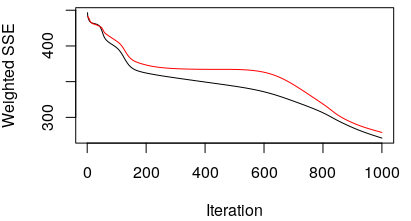
\includegraphics[scale=0.5]{01100503}
\caption{MLP $\gamma = 0.1$, $neuronas = 100,50$ y $ciclos = 10000$ pareja 3}
\end{figure} 

\par En comparación con el primer experimento realizado, la diferencia entre el porcentaje de acierto de entrenamiento y test ha disminuido. Aun así, la primera pareja de datos sigue presentando un comportamiento diferente al de las otras dos parejas. Según lo observado en la matriz de confusión se producen menos fallos a la hora de predecir, por tanto considero que es un mejor experimento que el anterior. A pesar de que la media de acierto en el caso de entrenamiento es menor, en caso de test es mayor, se sacrifica acierto en entrenamiento para saber generalizar mejor conjuntos nuevos.

%   EXPERIMENTO 3    %

\par \textbf{$\gamma = 0.01$, $neuronas = 10,10,5$ y $ciclos = 1000$}

\par Con una tasa de 0.01, 10 neuronas, 10 neuronas y 5 neuronas distribuidas en tres capas ocultas y 10000 ciclos tenemos los siguientes porcentajes de acierto:

\begin{table}[H]
\centering
\caption{MLP $\gamma = 0.01$, $neuronas = 10,10,5$ y $ciclos = 1000$}
\label{tb:tb3}
\begin{tabular}{lllll}
\hline
\multicolumn{1}{|l|}{Pareja} & Porcentaje de acierto entrenamiento & Porcentaje de acierto test  \\ \hline \hline
1                            & 0.263537906137184    & 0.246575342465753 \\
2                            & 0.253054101221641    & 0.267399267399267 \\
3                            & 0.253054101221641    & 0.259786476868327 \\
Media                        & 0.25654870286        & 0.25792036224     \\ \hline
\end{tabular}
\end{table}

\begin{figure}[H]
\centering
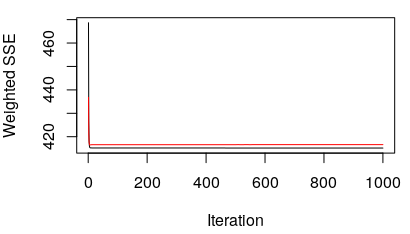
\includegraphics[scale=0.5]{001101051}
\caption{MLP $\gamma = 0.01$, $neuronas = 10,10,5$ y $ciclos = 1000$ pareja 1}
\end{figure} 

\begin{figure}[H]
\centering
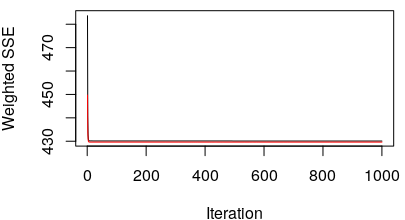
\includegraphics[scale=0.5]{001101052}
\caption{MLP $\gamma = 0.01$, $neuronas = 10,10,5$ y $ciclos = 1000$ pareja 2}
\end{figure} 

\begin{figure}[H]
\centering
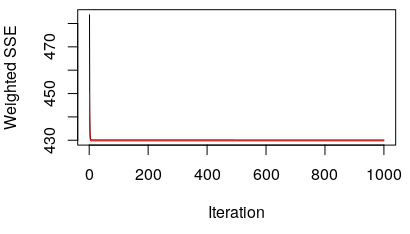
\includegraphics[scale=0.5]{001101053}
\caption{MLP $\gamma = 0.01$, $neuronas = 10,10,5$ y $ciclos = 1000$ pareja 3}
\end{figure} 

\par Como vemos, el resultado en este experimento es que las tres parejas tienen un comportamiento muy similar, el porcentaje de acierto tanto en test como en entrenamiento es muy parecido entre ellas, aunque es demasiado bajo como para considerarlo un buen experimento.

%   EXPERIMENTO 4    %

\par \textbf{$\gamma = 0.1$, $neuronas = 100,50,25$ y $ciclos = 1000$}

\par Con una tasa de 0.1, 100 neuronas, 50 neuronas y 25 neuronas distribuidas en tres capas ocultas y 10000 ciclos tenemos los siguientes porcentajes de acierto:

\begin{table}[H]
\centering
\caption{MLP $\gamma = 0.1$, $neuronas = 100,50,25$ y $ciclos = 1000$}
\label{tb:tb4}
\begin{tabular}{lllll}
\hline
\multicolumn{1}{|l|}{Pareja} & Porcentaje de acierto entrenamiento & Porcentaje de acierto test  \\ \hline \hline
1                            & 0.465703971119134    & 0.414383561643836 \\
2                            & 0.56195462478185     & 0.582417582417582 \\
3                            & 0.363001745200698    & 0.298932384341637 \\
Media                        & 0.46355344703        & 0.43191117613     \\ \hline
\end{tabular}
\end{table}

\begin{figure}[H]
\centering
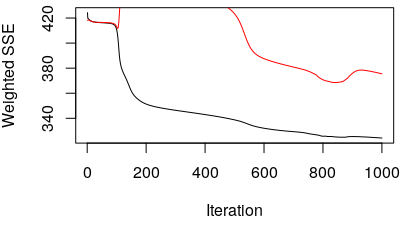
\includegraphics[scale=0.5]{0110050251}
\caption{MLP $\gamma = 0.1$, $neuronas = 100,50,25$ y $ciclos = 1000$ pareja 1}
\end{figure} 

\begin{figure}[H]
\centering
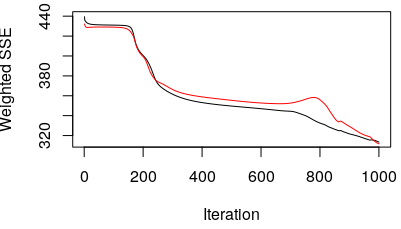
\includegraphics[scale=0.5]{0110050252}
\caption{MLP $\gamma = 0.1$, $neuronas = 100,50,25$ y $ciclos = 1000$ pareja 2}
\end{figure} 

\begin{figure}[H]
\centering
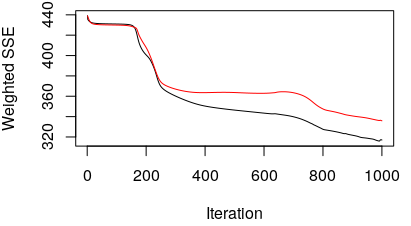
\includegraphics[scale=0.5]{0110050253}
\caption{MLP $\gamma = 0.1$, $neuronas = 100,50,25$ y $ciclos = 1000$ pareja 3}
\end{figure} 

\par El resultado observado es, de nuevo, que para la primera pareja de datos de entrenamiento y test el error del conjunto de test es más elevado que el de entrenamiento. El porcentaje de acierto es moderado pero estable relativamente.

%   EXPERIMENTO 5    %

\par \textbf{$\gamma = 0.1$, $neuronas = 100,50,25,12$ y $ciclos = 1000$}

\par Con una tasa de 0.1, 100 neuronas, 50 neuronas y 25 neuronas distribuidas en tres capas ocultas y 10000 ciclos tenemos los siguientes porcentajes de acierto:

\begin{table}[H]
\centering
\caption{MLP $\gamma = 0.1$, $neuronas = 100,50,25,12$ y $ciclos = 1000$}
\label{tb:tb5}
\begin{tabular}{lllll}
\hline
\multicolumn{1}{|l|}{Pareja} & Porcentaje de acierto entrenamiento & Porcentaje de acierto test  \\ \hline \hline
1                            & 0.263537906137184    & 0.246575342465753 \\
2                            & 0.253054101221641    & 0.267399267399267 \\
3                            & 0.253054101221641    & 0.259786476868327 \\
Media                        & 0.25654870286        & 0.25792036224     \\ \hline
\end{tabular}
\end{table}

\begin{figure}[H]
\centering
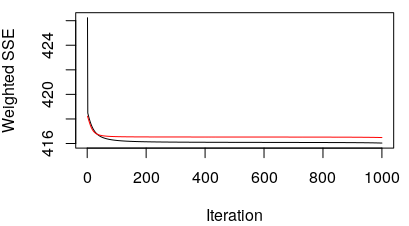
\includegraphics[scale=0.5]{011005025121}
\caption{MLP $\gamma = 0.1$, $neuronas = 100,50,25,12$ y $ciclos = 1000$ pareja 1}
\end{figure} 

\begin{figure}[H]
\centering
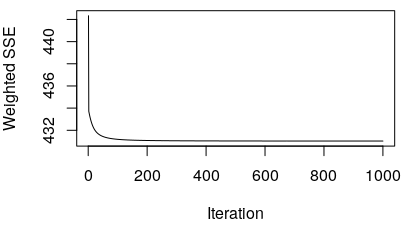
\includegraphics[scale=0.5]{011005025122}
\caption{MLP $\gamma = 0.1$, $neuronas = 100,50,25,12$ y $ciclos = 1000$ pareja 2}
\end{figure} 

\begin{figure}[H]
\centering
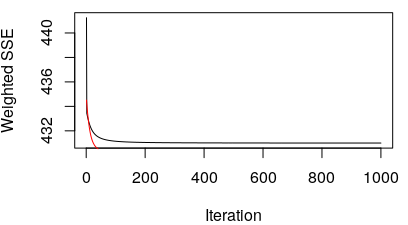
\includegraphics[scale=0.5]{011005025123}
\caption{MLP $\gamma = 0.1$, $neuronas = 100,50,25,12$ y $ciclos = 1000$ pareja 3}
\end{figure} 

\par Como vemos, el presente experimento presenta tasas de acierto bajas pero estables. Observando la matriz de confusión, se clasifican todos los patrones como uno de ellos, y por tanto el porcentaje de acierto es aproximadamente 1/4. Este experimento no es apropiado.

%   EXPERIMENTO 6    %

\par \textbf{$\gamma = 0.8$, $neuronas = 100$ y $ciclos = 1000$}

\par Con una tasa de 0.8, 100 neuronas en una capa oculta y 10000 ciclos tenemos los siguientes porcentajes de acierto:

\begin{table}[H]
\centering
\caption{MLP $\gamma = 0.8$, $neuronas = 100$ y $ciclos = 1000$}
\label{tb:tb6}
\begin{tabular}{lllll}
\hline
\multicolumn{1}{|l|}{Pareja} & Porcentaje de acierto entrenamiento & Porcentaje de acierto test  \\ \hline \hline
1                            & 0.846570397111913    & 0.424657534246575 \\
2                            & 0.478184991273996    & 0.47985347985348  \\
3                            & 0.696335078534031    & 0.651245551601424 \\
Media                        & 0.6736968223         & 0.5185855219      \\ \hline
\end{tabular}
\end{table}

\begin{figure}[H]
\centering
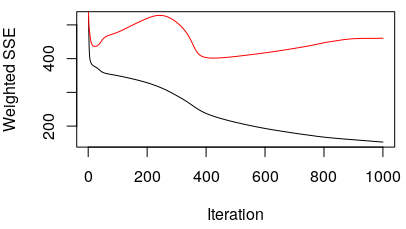
\includegraphics[scale=0.5]{081001}
\caption{MLP $\gamma = 0.8$, $neuronas = 100$ y $ciclos = 1000$ pareja 1}
\end{figure} 

\begin{figure}[H]
\centering
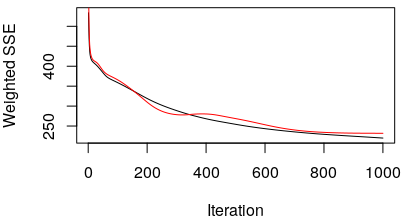
\includegraphics[scale=0.5]{081002}
\caption{MLP $\gamma = 0.8$, $neuronas = 100$ y $ciclos = 1000$ pareja 2}
\end{figure} 

\begin{figure}[H]
\centering
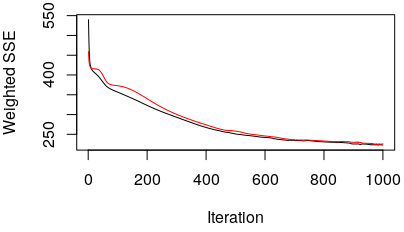
\includegraphics[scale=0.5]{081003}
\caption{MLP $\gamma = 0.8$, $neuronas = 100$ y $ciclos = 1000$ pareja 3}
\end{figure} 

\par Observando la matriz de confusión vemos que las predicciones se aproximan bastante bien a los valores reales, y además los porcentajes de aciertos son buenos. A pesar de todo el segundo experimento sigue ofreciendo mejores resultados. 

%%%%%%%%%%%%%%%%%%%%%%%%%%%%%%%%%%%%%%%%%%%%%%%%%%%%%%%%%%%%%%%%%%%%%%%%%%%%%%%
%                                      LVQ                                    %
%%%%%%%%%%%%%%%%%%%%%%%%%%%%%%%%%%%%%%%%%%%%%%%%%%%%%%%%%%%%%%%%%%%%%%%%%%%%%%%

\chapter{Learning Vector Quantization}

\par En este capítulo se va a explicar en primer lugar el algotitmo LVQ, una versión supervisada del método de Kohonen en la que se conoce de antemano el número de clases, clasificando por vecindad.

\section{Learning Vector Quantization (LVQ)}

\par Es un algoritmo supervisado de clasificación basado en prototipos. Inicialmente los prototipos se distribuyen aleatoriamente por el espacio de entrada, y una vez que la red se entrene, se obtiene la solución al problema de clasificación que consiste en la colocación final de los prototipos.

\par El entrenamiento de la red se lleva a cabo de tal forma que inicialmente la distribución aleatoria de los prototipos es alterada por la introducción de los ejemplos de entrenamiento.

\par Para realizar la clasificación de un patrón del conjunto de test, se introduce el ejemplo, se calcula su distancia a todos los prototipos y por último se etiqueta con la clase del prototipo más cercano.

\section{Experimentación realizada}

\par En cuanto a la experimentación realizada se ha probado con distintos números de prototipos, escogiendo números proporcionales al número de clases existentes. Se atenderá al porcentaje de acierto realizando la media entre las tres hojas de la validación cruzada y se escogerá el mejor experimento.


\par \underline{\textbf{Experimentaciones}}

%   EXPERIMENTO 1    %

\par \textbf{$20 prototipos$}

\par Escogiendo 20 prototipos el resultado que obtenemos es el siguiente:

\begin{table}[H]
\centering
\caption{LVQ $20 prototipos$}
\label{tb:tb21}
\begin{tabular}{lllll}
\hline
\multicolumn{1}{|l|}{Pareja} & Porcentaje de acierto \\ \hline \hline
1                            & 0.2397			     \\
2                            & 0.2466			     \\
3                            & 0.2432			     \\
Media                        & 0.24316666666         \\ \hline
\end{tabular}
\end{table}

\begin{figure}[H]
\centering
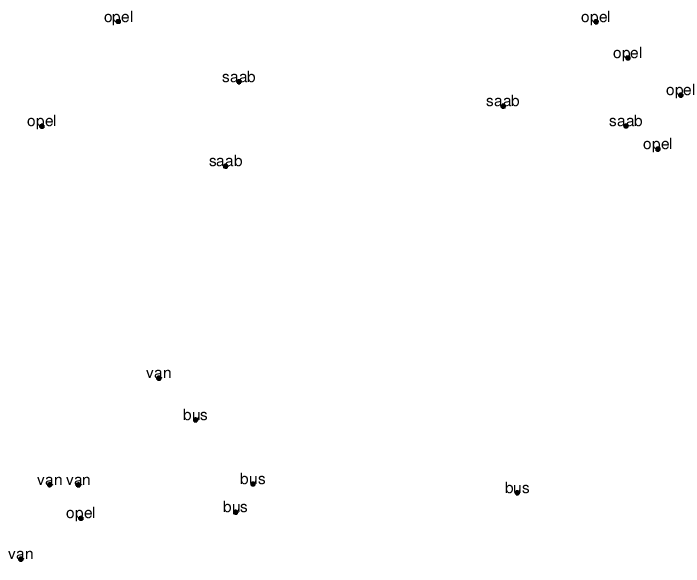
\includegraphics[scale=0.5]{lvq20p1}
\caption{LVQ $20 prototipos$ pareja 1}
\end{figure} 

\begin{figure}[H]
\centering
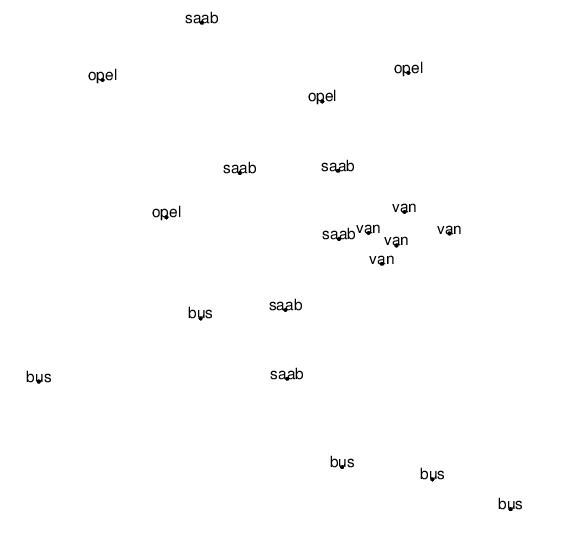
\includegraphics[scale=0.5]{lvq20p2}
\caption{LVQ $20 prototipos$ pareja 2}
\end{figure} 

\begin{figure}[H]
\centering
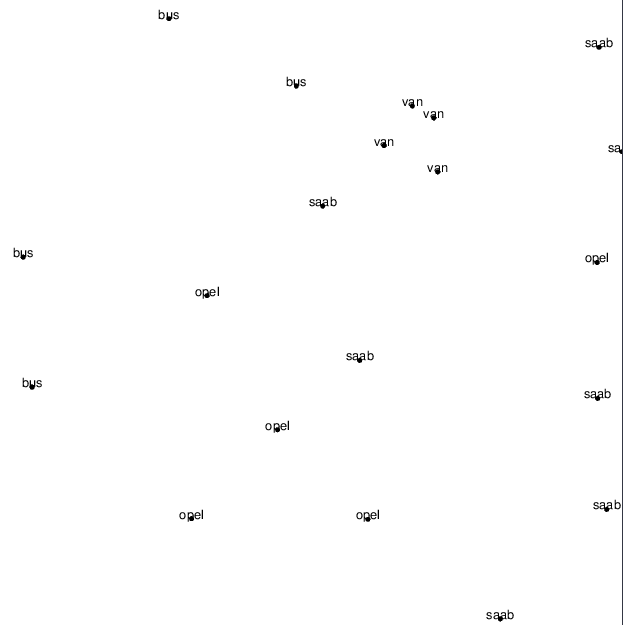
\includegraphics[scale=0.5]{lvq20p3}
\caption{LVQ $20 prototipos$ pareja 3}
\end{figure} 

\par Como se puede apreciar en las figuras, los resultados son bastante diferentes, la pareja 2 y 3 se aproxima bastante bien pero la primera pareja presenta resultados muy diferentes. La media del porcentaje de acierto es bastante bueno para entrenamiento pero no muy buena para test. Observando las matrices de confusión, la predicción no es muy buena para varias clases.







%%%%%%%%%%%%%%%%%%%%%%%%%%%%%%%%%%%%%%%%%%%%%%%%%%%%%%%%%%%%%%%%%%%%%%%%%%%%%%%
%                         Mapas autoorganizados de Kohonen                    %
%%%%%%%%%%%%%%%%%%%%%%%%%%%%%%%%%%%%%%%%%%%%%%%%%%%%%%%%%%%%%%%%%%%%%%%%%%%%%%%

\chapter{Mapas autoorganizados de Kohonen}



%%%%%%%%%%%%%%%%%%%%%%%%%%%%%%%%%%%%%%%%%%%%%%%%%%%%%%%%%%%%%%%%%%%%%%%%%%%%%%%
%                                 CONCLUSIONES                                %
%%%%%%%%%%%%%%%%%%%%%%%%%%%%%%%%%%%%%%%%%%%%%%%%%%%%%%%%%%%%%%%%%%%%%%%%%%%%%%%

\chapter{Conclusiones}

\par Analizados ambos modelos, estamos en disposición de valorar objetivamente cual de ellos da mejor resultado para el problema que teníamos que resolver: para ello veamos los dos modelos elegidos para cada tipo, y también la tabla de resultados de cada uno de los dos modelos. La diferencia entre ambos modelos es que en Adaline teníamos la posibilidad de modificar ciclos y tasa de aprendizaje mientras que en Perceptrón Multicapa hemos visto que además se pueden añadir capas de neuronas ocultas para hacer el modelo más complejo. El error de test que obtenemos en el mejor modelo escogido por Adaline es de 0.019147481314295 mientras que el error de test que obtenemos en el mejor modelo escogido MLP es de 0.00569856426934457. Como vemos resulta evidente que el error mejora significativamente en un factor de $\frac{1}{4}$ aproximadamente. Consideramos entonces que una red MLP aproxima mejor y es capaz de generalizar mejor en este caso concreto, aunque hay que tener cautela porque es fácil dejarse llevar y añadir las suficientes capas para que MLP aproxime exactamente el conjunto de entrenamiento, que como ya hemos visto en \ref{fig:10050012000tan} no nos lleva más que a una red que posteriormente fallará en la generalización de otros conjuntos de datos.

\par Es importante resaltar que aunque parezca que la diferencia es mínima en cuanto se "desnormalizan" los datos vemos que algunas salidas tanto en \ref{fig:bestmlp} como en \ref{fig:bestadaline} presentan errores de una magnitud bastante importante, y que en estos casos nuestras redes fallan en su generalización.

\par En cuanto a la práctica en general, pienso que ha habido problemas de rendimiento tanto en el script en R como en mi programa en PHP debido a que el proceso de aprendizaje si los ciclos son muy elevados he llegado a ver ejecuciones de veinte minutos. Lo cual ha provocado tener que invertir más tiempo en la práctica. Sería bueno plantearse mejorar el rendimiento de estos programas aunque se entiende que no es el objetivo principal.

%%%%%%%%%%%%%%%%%%%%%%%%%%%%%%%%%%%%%%%%%%%%%%%%%%%%%%%%%%%%%%%%%%%%%%%%%%%%%%%
%                                BIBLIOGRAFÍA                                 %
%%%%%%%%%%%%%%%%%%%%%%%%%%%%%%%%%%%%%%%%%%%%%%%%%%%%%%%%%%%%%%%%%%%%%%%%%%%%%%%

\begin{thebibliography}{10}


\bibitem{KEEL}
   Conjunto de datos de siluetas de vehículos, 
   \newblock Knowledge Extraction based on Evolutionary Learning. 
   \newblock Obtenido de
   \url{http://sci2s.ugr.es/keel/dataset.php?cod=68}.

\bibitem{MLP}
   Peceptrón Multicapa, 
   \newblock Inés M. Galván y José Mª Valls.
   \newblock Obtenido de
   \url{http://ocw.uc3m.es/ingenieria-informatica/redes-de-neuronas-artificiales/transparencias/material-de-clase.-tema-3/view}.

\bibitem{LVQ}
   Learning Vector Quantization, 
   \newblock Inés M. Galván y José Mª Valls.
   \newblock Obtenido de
   \url{http://ocw.uc3m.es/ingenieria-informatica/redes-de-neuronas/transparencias/LVQ.pdf/view}.

   

\end{thebibliography}
\cleardoublepage

%%%%%%%%%%%%%%%%%%%%%%%%%%%%%%%%%%%%%%%%%%%%%%%%%%%%%%%%%%%%%%%%%%%%%%%%%%%%%%%
%                              FI DEL DOCUMENT                                %
%%%%%%%%%%%%%%%%%%%%%%%%%%%%%%%%%%%%%%%%%%%%%%%%%%%%%%%%%%%%%%%%%%%%%%%%%%%%%%%

\end{document}
